\documentclass[english,serif,mathserif,xcolor=pdftex,dvipsnames,table]{beamer}
\usetheme{gc3}

\usepackage[T1]{fontenc}
\usepackage[utf8]{inputenc}
\usepackage{babel}

\usepackage{gc3}

\title[Introduction]{%
  GC3Pie basics
}
\author[R. Murri, S3IT UZH]{%
  Riccardo Murri \texttt{<riccardo.murri@uzh.ch>}
  \\[1ex]
  \emph{S3IT: Services and Support for Science IT}
  \\[1ex]
  University of Zurich
}
\date{July~11--14, 2016}

\begin{document}

% title frame
\maketitle

\section{Concepts and glossary}
\part{Concepts and glossary}

\begin{frame}
\frametitle{Parts of GC3Pie}

  GC3Pie consists of three main components:

  \begin{block}{GC3Libs:} Python library for controlling the life-cycle of computational job collections. \end{block}
  \begin{block}{GC3Utils:} This is a small set of low-level utilities exposing the main functionality provided by GC3Libs. \end{block}
  \begin{block}{GC3Apps:} A collection of driver scripts to run large job campaigns. \end{block}
\end{frame}

\begin{frame}
  \frametitle{GC3Pie glossary: Application}
  \begin{quote}
    GC3Pie runs \alert<2-3>{user applications}
    \\
    on clusters and IaaS cloud resources
  \end{quote}

  \uncover<2-3>{
    \+ \alert<2>{An \texttt{Application} is just a command to execute.}

    \+
    \only<2>{If you can run it in the terminal, \\ you can run it in GC3Pie.}
    \only<3>{
      \alert<3>{A single execution of an \texttt{Application} \\ is indeed called a \texttt{Run}.}

      \+ (Other systems might call this a ``job''.)
    }
  }
\end{frame}


\begin{frame}
  \frametitle{GC3Pie glossary: Task}
  \begin{quote}
    GC3Pie \alert{runs} user applications
    \\
    on clusters and IaaS cloud resources
  \end{quote}

  \+ More generally, GC3Pie runs \texttt{Task}s.

  \+ \texttt{Task}s are a superset of applications,
  \\ in that they include workflows.

  %\+ \hyperlink{workflows}{\beamergotobutton{More on this later!}}
\end{frame}


\begin{frame}
  \frametitle{GC3Pie glossary: Resources}
  \begin{quote}
    GC3Pie runs user applications
    \\
    on clusters and IaaS cloud \alert{resources}
  \end{quote}

  \+ \alert{\texttt{Resource}s are the computing infrastructures \\ where GC3Pie executes applications.}

  \+ Resources include: your laptop, the ``Hydra'' cluster, the Science Cloud, Amazon AWS.
\end{frame}


\section{Scaffolding}
\part{Workflow scaffolding}

\begin{frame}[fragile]
  \frametitle{Let's start coding!}
  \begin{columns}
    \begin{column}{0.7\linewidth}
\begin{python}
from gc3libs.cmdline \
  import SessionBasedScript

if __name__ == '__main__':
  import ex2a
  ex2a.AScript().run()

class AScript(SessionBasedScript):
  """
  Minimal workflow scaffolding.
  """
  def __init__(self):
    super(AScript, self).__init__(
        version='1.0')
  def new_tasks(self, extra):
    return []
\end{python}
    \end{column}
    \begin{column}{0.3\linewidth}
      \href{https://raw.githubusercontent.com/uzh/gc3pie/master/docs/programmers/tutorials/workflows/solutions/ex2a.py}{Download} this code into a file named \texttt{ex2a.py}

      \+
      Open it in your favorite text editor.
    \end{column}
  \end{columns}
\end{frame}


\begin{frame}[fragile]
  \begin{exercise*}[2.A]

    \+
    \href{https://raw.githubusercontent.com/uzh/gc3pie/master/docs/programmers/tutorials/workflows/solutions/ex2a.py}{Download this code} into a file named \texttt{ex2a.py}

    \begin{enumerate}
    \item Run the following command:
\begin{sh}
> python ex2a.py --help
\end{sh}
        Where does the program description in the help text come from?
        Is there anything weird in other parts of the help text?

    \item Run the following command:
\begin{sh}
> python ex2a.py
\end{sh}
        What happens?
      \end{enumerate}
  \end{exercise*}
\end{frame}


\begin{frame}[fragile]
  \begin{columns}[t]
    \begin{column}{0.7\linewidth}
\begin{python}
from gc3libs.cmdline \
  import SessionBasedScript

~\HL{if \_\_name\_\_ == '\_\_main\_\_':}~
  ~\HL{import ex2a}~
  ~\HL{ex2a.AScript().run()}~

class AScript(SessionBasedScript):
  """
  Minimal workflow scaffolding.
  """
  def __init__(self):
    super(AScript, self).__init__(
        version='1.0')
  def new_tasks(self, extra):
    return []
\end{python}
    \end{column}
    \begin{column}{0.4\linewidth}
      \begin{flushright}
        These lines are needed in every session-based script.

        \+
        See \href{https://github.com/uzh/gc3pie/issues/95}{issue 95} for details.
      \end{flushright}
    \end{column}
  \end{columns}
\end{frame}


\begin{frame}[fragile]
  \begin{columns}[t]
    \begin{column}{0.7\linewidth}
\begin{python}
from gc3libs.cmdline \
  import SessionBasedScript

if __name__ == '__main__':
  import ~\HL{ex2a}~
  ~\HL{ex2a}~.AScript().run()

class AScript(SessionBasedScript):
  """
  Minimal workflow scaffolding.
  """
  def __init__(self):
    super(AScript, self).__init__(
        version='1.0')
  def new_tasks(self, extra):
    return []
\end{python}
    \end{column}
    \begin{column}{0.4\linewidth}
      \begin{flushright}
        For this to work, it is \textbf{needed} that this is the
        actual file name.
      \end{flushright}
    \end{column}
  \end{columns}
\end{frame}


\begin{frame}[fragile]
  \begin{columns}
    \begin{column}{0.7\linewidth}
\begin{python}
from gc3libs.cmdline \
  import SessionBasedScript

if __name__ == '__main__':
  import ex2a
  ex2a.AScript().run()

class AScript(SessionBasedScript):
  """
  ~\HL{Minimal workflow scaffolding.}~
  """
  def __init__(self):
    super(AScript, self).__init__(
        version='1.0')
  def new_tasks(self, extra):
    return []
\end{python}
    \end{column}
    \begin{column}{0.4\linewidth}
      \begin{flushright}
        This is the \\ program's help text!
      \end{flushright}
    \end{column}
  \end{columns}
\end{frame}


\begin{frame}[fragile]
  \begin{columns}
    \begin{column}{0.7\linewidth}
\begin{python}
from gc3libs.cmdline \
  import SessionBasedScript

if __name__ == '__main__':
  import ex2a
  ex2a.AScript().run()

class AScript(SessionBasedScript):
  """
  Minimal workflow scaffolding.
  """
  def __init__(self):
    super(AScript, self).__init__(
      ~\HL{version='1.0'}~)
  def new_tasks(self, extra):
    return []
\end{python}
    \end{column}
    \begin{column}{0.4\linewidth}
      \begin{flushright}
        A version number \\ is \textbf{mandatory}.
      \end{flushright}
    \end{column}
  \end{columns}
\end{frame}


\begin{frame}[fragile]
  \begin{columns}
    \begin{column}{0.7\linewidth}
\begin{python}
from gc3libs.cmdline \
  import SessionBasedScript

if __name__ == '__main__':
  import ex2a
  ex2a.AScript().run()

class AScript(SessionBasedScript):
  """
  Minimal workflow scaffolding.
  """
  def __init__(self):
    super(AScript, self).__init__(
        version='1.0')
  def new_tasks(self, extra):
    ~\HL{return []}~
\end{python}
    \end{column}
    \begin{column}{0.4\linewidth}
      \begin{flushright}
        \textbf{This is the core of the script.}

        \+
        Return a list of \texttt{Application} objects, that GC3Pie will execute.
      \end{flushright}
    \end{column}
  \end{columns}
\end{frame}


\section{Applications}
\part{The \texttt{Application} object}

\begin{frame}
  \frametitle{Specifying commands to run, I}

  You need to ``describe'' an application to GC3Pie, in order for
  GC3Pie to use it.

  \+
  This ``description'' is a blueprint from which many actual
  command instances can be created.

  \+
  (A few such ``descriptions'' are already part of the core library.)
\end{frame}


\begin{frame}
  \frametitle{GC3Pie application model}

  In GC3Pie, an application ``description'' is an object of the
  \texttt{gc3libs.Application} class (or subclasses thereof).

  \+
  At a minimum: provide application-specific command-line invocation.

  \+
  Advanced users can customize pre- and post-processing, react on
  state transitions, set computational requirements based on input
  files, influence scheduling.  (This is standard OOP: subclass and
  override a method.)
\end{frame}


\begin{frame}[fragile]
\frametitle{A basic example: grayscaling}
\begin{sh}
$ convert lena.jpg -colorspace gray lena-gray.jpg
\end{sh}%$
\begin{tabular}{ccc}
  {
\includegraphics[width=0.4\linewidth]{fig/lena.jpg}}
  &
  {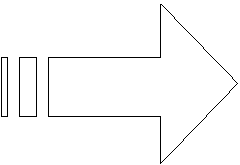
\includegraphics[width=0.1\linewidth,totalheight=0.45\textheight]{fig/arrow.pdf}}
  &
  {\includegraphics[width=0.4\linewidth]{fig/gray-lena.jpg}}
\end{tabular}

\end{frame}


\begin{frame}[fragile]
\frametitle{Grayscaling example, I}

  Here is how you would tell GC3Pie \\ to run that command-line.

\begin{python}
from gc3libs import Application

class GrayscaleApp(Application):
  """Convert an image file to grayscale."""
  def __init__(self, img):
    inp = basename(img)
    out = "gray-" + inp
    Application.__init__(
      self,
      arguments=[
        "convert", inp, "-colorspace", "gray", out],
      inputs=[img],
      outputs=[out],
      output_dir="grayscale.d",
      stdout="stdout.txt")
\end{python}
\end{frame}


\begin{frame}[fragile]
\frametitle{Always inherit from Application}

  Your application class must inherit from class \texttt{gc3libs.Application}
  \+
\begin{python}
~\HL{from gc3libs import Application}~

class GrayscaleApp~\HL{(Application)}~:
  """Convert an image file to grayscale."""
  def __init__(self, img):
    inp = basename(img)
    out = "gray-" + inp
    Application.__init__(
      self,
      arguments=[
        "convert", inp, "-colorspace", "gray", out],
      inputs=[img],
      outputs=[out],
      output_dir="grayscale.d",
      stdout="stdout.txt")
\end{python}
\end{frame}


\begin{frame}[fragile]
  \frametitle{The \texttt{arguments} parameter, I}

  The \texttt{arguments=} parameter is the actual command-line to be invoked.

  \+
\begin{python}
class GrayscaleApp(Application):
  """Convert an image file to grayscale."""
  def __init__(self, img):
    inp = basename(img)
    out = "gray-" + inp
    Application.__init__(
      self,
      ~\HL{arguments=[}~
        ~\HL{"convert", inp, "-colorspace", "gray", out],}~
      inputs=[img],
      outputs=[out],
      output_dir="grayscale.d",
      stdout="stdout.txt")
\end{python}
\end{frame}

\begin{frame}[fragile]
\frametitle{The \texttt{arguments} parameter, II}

The first item in the \texttt{arguments} list is the name or path to the command to run.

  \+
\begin{python}
class GrayscaleApp(Application):
  """Convert an image file to grayscale."""
  def __init__(self, img):
    inp = basename(img)
    out = "gray-" + inp
    Application.__init__(
      self,
      arguments=[
        ~\HL{"convert"}~, inp, "-colorspace", "gray", out],
      inputs=[img],
      outputs=[out],
      output_dir="grayscale.d",
      stdout="stdout.txt")
\end{python}
\end{frame}

\begin{frame}[fragile]
\frametitle{The \texttt{arguments} parameter, III}

The rest of the list are arguments to the program, as you would type
them at the shell prompt.

  \+
\begin{python}
class GrayscaleApp(Application):
  """Convert an image file to grayscale."""
  def __init__(self, img):
    inp = basename(img)
    out = "gray-" + inp
    Application.__init__(
      self,
      arguments=[
        "convert", ~\HL{inp, "-colorspace", "gray", out}~],
      inputs=[img],
      outputs=[out],
      output_dir="grayscale.d",
      stdout="stdout.txt")
\end{python}
\end{frame}


\begin{frame}[fragile]
\frametitle{The \texttt{inputs} parameter, I}

The \texttt{inputs} parameter holds a list of files that you want to
\emph{copy} to the location where the command is executed. (Remember:
this might be a remote computer!)

  \+
\begin{python}
class GrayscaleApp(Application):
  """Convert an image file to grayscale."""
  def __init__(self, img):
    inp = basename(img)
    out = "gray-" + inp
    Application.__init__(
      self,
      arguments=[
        "convert", inp, "-colorspace", "gray", out],
      ~\HL{inputs=[img]}~,
      outputs=[out],
      output_dir="grayscale.d",
      stdout="stdout.txt")
\end{python}
\end{frame}


\begin{frame}[fragile]
  \frametitle{The \texttt{inputs} parameter, II}

  Input files retain their name during the copy, \\ but not the entire path.

  \+
  For example:
  \begin{python}
    inputs = [
      '/home/rmurri/values.dat',
      '/home/rmurri/stats.csv',
      ]
  \end{python}
  will make files \emph{values.dat} and \emph{stats.csv} available in
  the command execution directory.

\end{frame}


\begin{frame}[fragile]
  \frametitle{The \texttt{inputs} parameter, III}

  You need to pass the full path name into the
  \texttt{inputs} list, but use only the ``base name'' in the command
  invocation.

\begin{python}
class GrayscaleApp(Application):
  """Convert an image file to grayscale."""
  def __init__(self, img):
    ~\HL{inp = basename(img)}~
    out = "gray-" + inp
    Application.__init__(
      self,
      arguments=[
        "convert", ~\HL{inp}~, "-colorspace", "gray", out],
      inputs=[~\HL{img}~],
      outputs=[out],
      output_dir="grayscale.d",
      stdout="stdout.txt")
\end{python}
\end{frame}


\begin{frame}[fragile]
\frametitle{The \texttt{outputs} parameter, I}

The \texttt{outputs} argument list files that should be copied from
the command execution directory back to your computer.

  \+
\begin{python}
class GrayscaleApp(Application):
  """Convert an image file to grayscale."""
  def __init__(self, img):
    inp = basename(img)
    out = "gray-" + inp
    Application.__init__(
      self,
      arguments=[
        "convert", inp, "-colorspace", "gray", out],
      inputs=[img],
      ~\HL{outputs=[out]}~,
      output_dir="grayscale.d",
      stdout="stdout.txt")
\end{python}
\end{frame}


\begin{frame}[fragile]
  \frametitle{The \texttt{outputs} parameter, II}

  Output file names are \emph{relative to the execution directory}.
  For example:
  \begin{python}
    outputs = ['result.dat', 'program.log']
  \end{python}

  \+
  (Contrast with input files, which must be specified by
  \emph{absolute path}, e.g., \texttt{/home/rmurri/values.dat})

  \+
  Any file with the given name that is found in the execution
  directory will be copied back. (\emph{Where?} See next slides!)

  \+
  If an output file is \emph{not} found, this is \emph{not} an
  error. In other words, \textbf{output files are optional}.
\end{frame}


\begin{frame}[fragile]
\frametitle{The \texttt{output\_dir} parameter, I}

The \lstinline|output_dir| parameter specifies where output filess
will be downloaded.

\+
\begin{python}
class GrayscaleApp(Application):
  """Convert an image file to grayscale."""
  def __init__(self, img):
    inp = basename(img)
    out = "gray-" + inp
    Application.__init__(
      self,
      arguments=[
        "convert", inp, "-colorspace", "gray", out],
      inputs=[img],
      outputs=[out],
      ~\HL{output\_dir="grayscale.d"}~,
      stdout="stdout.txt")
\end{python}
\end{frame}


\begin{frame}[fragile]
  \frametitle{The \emph{output\_dir} parameter, II}

  By default, GC3Pie does not overwrite an existing output directory:
  it will move the existing one to a backup name.

  \+
  So, if \texttt{grayscale.d} already exists, GC3Pie will:
  \begin{enumerate}
  \item rename it to \lstinline|grayscale.d.~1~|
  \item create a new directory \texttt{grayscale.d}
  \item download output files into the new directory
  \end{enumerate}
\end{frame}


\begin{frame}[fragile]
\frametitle{The \texttt{stdout} parameter}

This specifies that the command's \texttt{standard output} should be
saved into a file named \texttt{stdout.txt} and retrieved along with
the other output files.

  \+
\begin{python}
class GrayscaleApp(Application):
  """Convert an image file to grayscale."""
  def __init__(self, img):
    inp = basename(img)
    out = "gray-" + inp
    Application.__init__(
      self,
      arguments=[
        "convert", inp, "-colorspace", "gray", out],
      inputs=[img],
      outputs=[out],
      output_dir="grayscale.d",
      ~\HL{stdout="stdout.txt"}~)
\end{python}
\end{frame}


\begin{frame}[fragile]
\frametitle{(The \texttt{stderr} parameter)}

There's a corresponding \texttt{stderr} option for the command's
\emph{standard error} stream.

\begin{python}
class GrayscaleApp(Application):
  """Convert an image file to grayscale."""
  def __init__(self, img):
    inp = basename(img)
    out = "gray-" + inp
    Application.__init__(
      self,
      arguments=[
        "convert", inp, "-colorspace", "gray", out],
      inputs=[img],
      outputs=[out],
      output_dir="grayscale.d",
      stdout="stdout.txt",
      ~\HL{stderr="stderr.txt"}~)
\end{python}
\end{frame}


\begin{frame}
  \frametitle{Mixing \texttt{stdout} and \texttt{stderr} capture}

  You can specify \textbf{either one} of the \texttt{stdout} and
  \texttt{stderr} parameters, \textbf{or both}.

  \+
  If you give both, and they have the same value, then
  \texttt{stdout} and \texttt{stderr} will be intermixed just as they
  are in normal screen output.
\end{frame}


\begin{frame}[fragile]
  \frametitle{Let's run!}
  In order for a session-based script to execute something, its
  \texttt{new\_tasks()} method must return a list of
  \texttt{Application} objects to run.

\+
\begin{python}
class AScript(SessionBasedScript):
  # ...
  def new_tasks(self, extra):
    # `self.param.args' is the list
    # of command-line arguments
    input_file = self.params.args[0]
    app = GrayscaleApp(input_file)
    return [app]
\end{python}
\end{frame}

\begin{frame}[fragile]
  \small

  \begin{exercise*}[2.B]

    \+
    Edit the \texttt{ex2a.py} file: insert the code to define the
    \href{https://raw.githubusercontent.com/uzh/gc3pie/master/docs/programmers/tutorials/workflows/grayscale_app.py}{\texttt{GrayscaleApp}}
    application, and modify the \texttt{new\_tasks()} method to return
    one instance of it (as in the previous slide).

    \+
    Can you convert the \href{https://raw.githubusercontent.com/uzh/gc3pie/master/docs/programmers/tutorials/workflows/lena.jpg}{\texttt{lena.jpg}} file to gray-scale using
    this GC3Pie script?

    \+ \footnotesize
    {\em (You can download the code for \texttt{GrayscaleApp} and the ``Lena'' image file from
    \href{https://raw.githubusercontent.com/uzh/gc3pie/master/docs/programmers/tutorials/workflows/}{this
      URL}.)}
  \end{exercise*}

  \+
  \begin{exercise*}[2.C]

    Edit the script from Exercise 2.B above and add the ability to
    convert multiple files: for each file name given on the command
    line, an instance of \texttt{GrayscaleApp} should be run.
  \end{exercise*}
\end{frame}


\begin{frame}[fragile]
\frametitle{Application lifecycle}

\begin{columns}[c]
  \begin{column}{0.5\textwidth}
\begin{lstlisting}[basicstyle=\footnotesize\ttfamily,keywordstyle=\normalfont]
$ ./grayscale.py lena.jpg
~\em [\ldots]~
         NEW  1/1  (100.0%)
     RUNNING  0/1   (0.0%)
     STOPPED  0/1   (0.0%)
   SUBMITTED  0/1   (0.0%)
  TERMINATED  0/1   (0.0%)
 TERMINATING  0/1   (0.0%)
     UNKNOWN  0/1   (0.0%)
       total  1/1  (100.0%)
\end{lstlisting}%$
  \end{column}
  \begin{column}{0.5\textwidth}
    \raggedleft
    \texttt{Application} objects can be in one of several states.

    \+
    (A session-based script prints a table of all managed applications and their states.)
  \end{column}
\end{columns}

\+
\begin{columns}[c]
  \begin{column}{0.5\textwidth}
\begin{lstlisting}[basicstyle=\footnotesize\ttfamily]
>>> print(app.execution.state)
'TERMINATED'
\end{lstlisting}
  \end{column}
  \begin{column}{0.5\textwidth}
    \raggedleft
    The current state is stored in the \texttt{.execution.state} instance attribute.
  \end{column}
\end{columns}

\+
\begin{references}
  \tiny
  \url{http://gc3pie.readthedocs.io/en/master/programmers/api/gc3libs.html#gc3libs.Run.state}
\end{references}
\end{frame}


\begin{frame}[fragile]
\frametitle{Application lifecycle: state NEW}

\begin{columns}[c]
  \begin{column}{0.5\textwidth}
    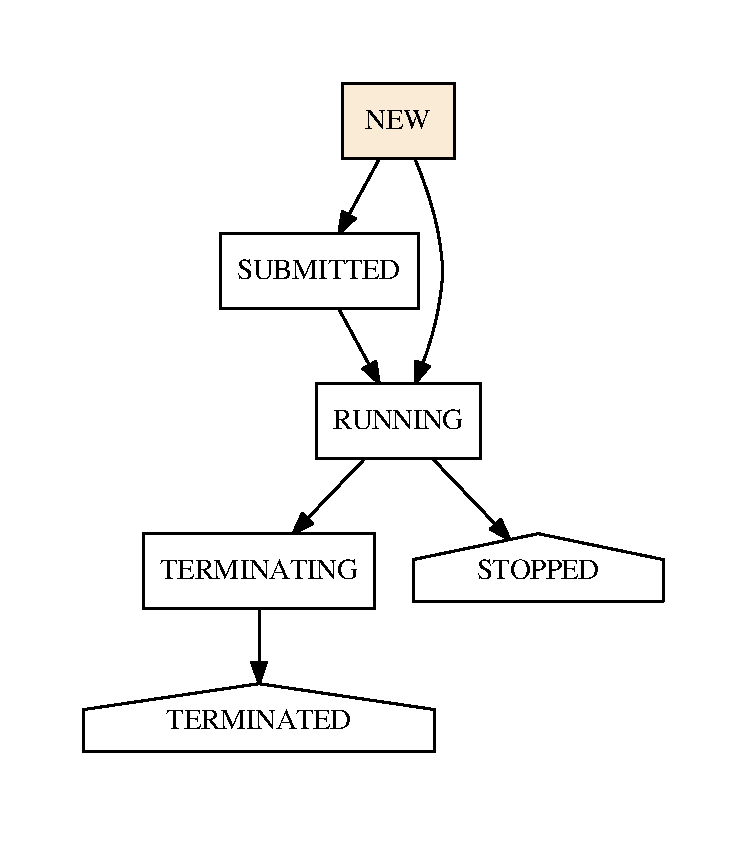
\includegraphics[height=0.7\textheight]{fig/states-NEW}
  \end{column}
  \begin{column}{0.5\textwidth}
    \raggedleft
    \textbf{NEW} is the state of ``just created'' Application objects.

    \+
    The Application has not yet been sent off to a compute
    resource: it only exists locally.
  \end{column}
\end{columns}
\end{frame}


\begin{frame}[fragile]
\frametitle{Application lifecycle: state SUBMITTED}

\begin{columns}[c]
  \begin{column}{0.5\textwidth}
    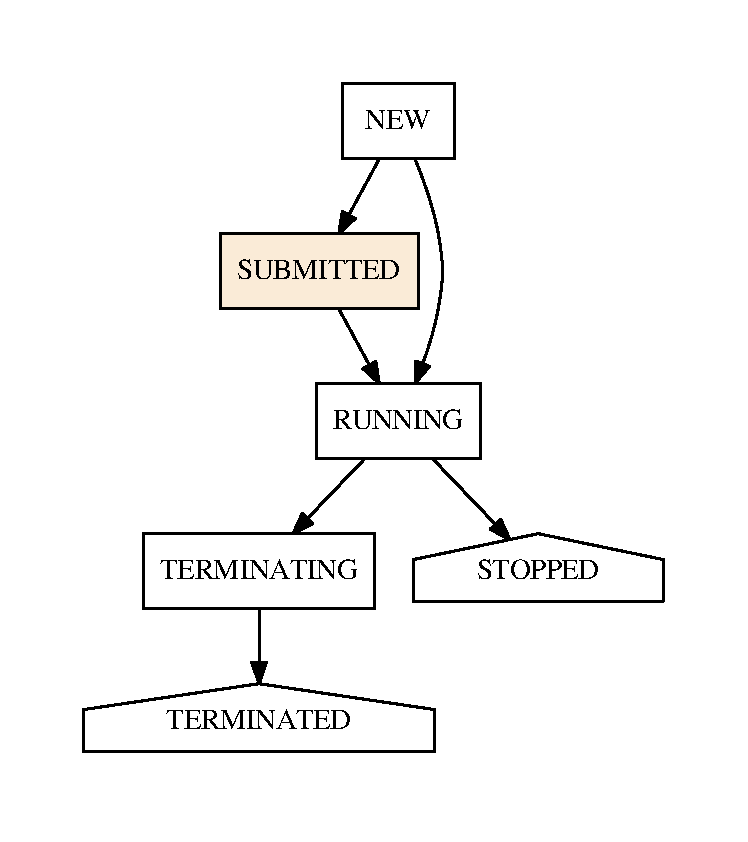
\includegraphics[height=0.7\textheight]{fig/states-SUBMITTED}
  \end{column}
  \begin{column}{0.5\textwidth}
    \raggedleft
    \emph{SUBMITTED} applications have been successfully sent to a
    computational resource.

    \+
    (The transition to \emph{RUNNING} happens automatically, as we
    do not control the remote execution.)
  \end{column}
\end{columns}
\end{frame}


\begin{frame}[fragile]
\frametitle{Application lifecycle: state RUNNING}

\begin{columns}[c]
  \begin{column}{0.5\textwidth}
    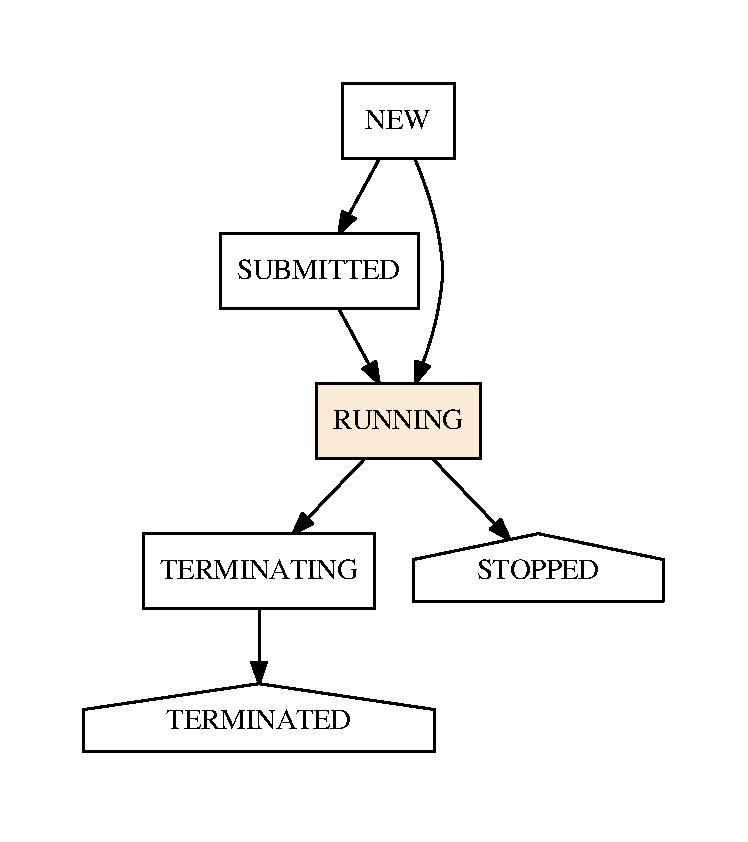
\includegraphics[height=0.7\textheight]{fig/states-RUNNING}
  \end{column}
  \begin{column}{0.5\textwidth}
    \raggedleft
    \emph{RUNNING} state happens when the computational job associated to an
    application starts executing on the computational resource.
  \end{column}
\end{columns}
\end{frame}


\begin{frame}[fragile]
\frametitle{Application lifecycle: state STOPPED}

\begin{columns}[c]
  \begin{column}{0.5\textwidth}
    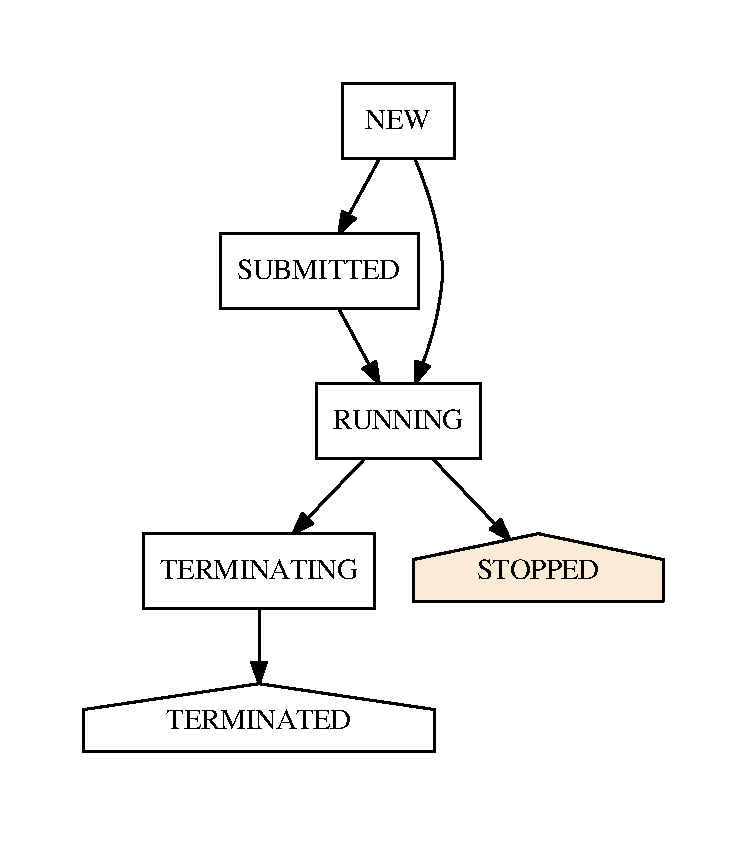
\includegraphics[height=0.7\textheight]{fig/states-STOPPED}
  \end{column}
  \begin{column}{0.5\textwidth}
    \raggedleft
    A task is in \emph{STOPPED} state when its execution has been
    blocked at the remote site and GC3Pie cannot recover
    automatically.

    \+
    User or sysadmin intervention is required for a task to get out
    of \emph{STOPPED} state.
  \end{column}
\end{columns}
\end{frame}


\begin{frame}[fragile]
\frametitle{Application lifecycle: state UNKNOWN}

\begin{columns}[c]
  \begin{column}{0.5\textwidth}
    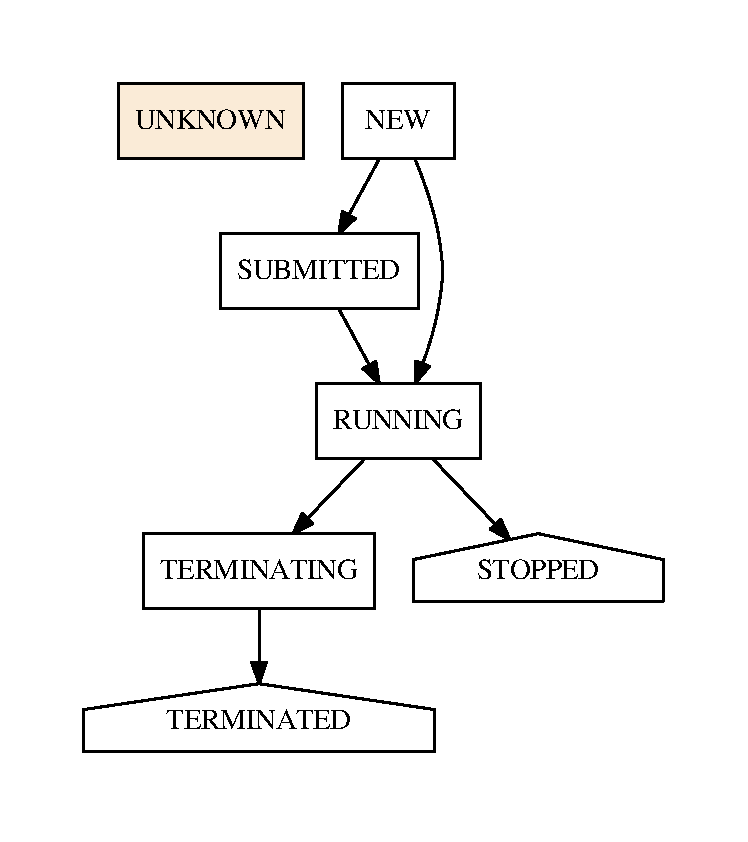
\includegraphics[height=0.7\textheight]{fig/states-UNKNOWN}
  \end{column}
  \begin{column}{0.5\textwidth}
    \raggedleft
    A task is in \emph{UNKNOWN} state when GC3Pie can no
    longer monitor it at the remote site.

    \+
    (As this might be due to network failures, jobs \emph{can} get
    out of \emph{UNKNOWN} automatically.)
  \end{column}
\end{columns}
\end{frame}


\begin{frame}[fragile]
\frametitle{Application lifecycle: state TERMINATING}

\begin{columns}[c]
  \begin{column}{0.5\textwidth}
    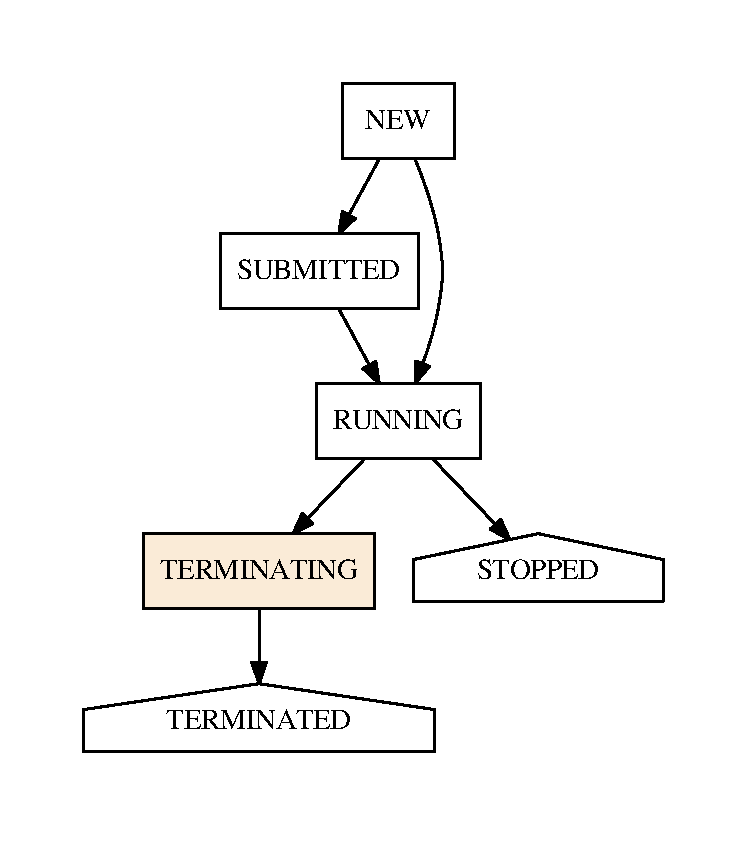
\includegraphics[height=0.7\textheight]{fig/states-TERMINATING}
  \end{column}
  \begin{column}{0.5\textwidth}
    \raggedleft
    \emph{TERMINATING} state when a computational job has finished
    running, for whatever reason.

    \+
    (Transition to \emph{TERMINATED} only happens when \texttt{fetch\_output} is called.)
  \end{column}
\end{columns}
\end{frame}


\begin{frame}[fragile]
\frametitle{Application lifecycle: state TERMINATED}

\begin{columns}[c]
  \begin{column}{0.5\textwidth}
    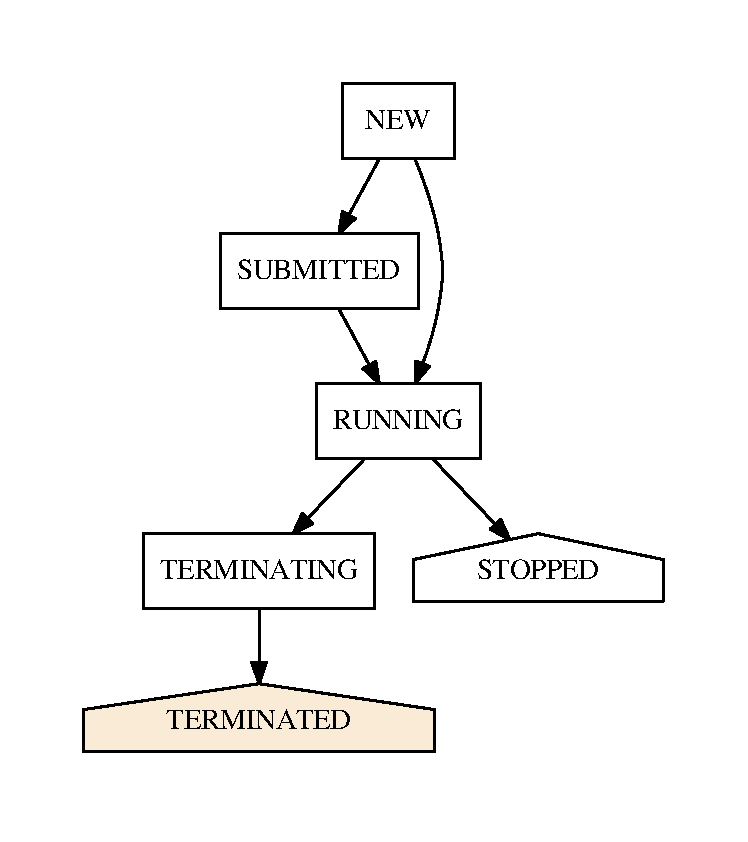
\includegraphics[height=0.7\textheight]{fig/states-TERMINATED}
  \end{column}
  \begin{column}{0.5\textwidth}
    \raggedleft
    A job is \emph{TERMINATED} when its final output has been
    retrieved and is available locally.

    \+
    The exit code of \emph{TERMINATED} jobs can be inspected to
    find out whether the termination was successful or unsuccessful,
    or if the program was forcibly ended.
  \end{column}
\end{columns}
\end{frame}


\begin{frame}[fragile]
  \frametitle{Post-processing features, I}

  When the remote computation is done, the \texttt{terminated} method
  of the application instance is called.

  \+
  The path to the output directory is available as
  \lstinline|self.output_dir|; if \texttt{stdout} and \texttt{srderr}
  have been captured, the paths to the capture files are available as
  \lstinline|self.stdout| and \lstinline|self.stderr|.
\end{frame}


\begin{frame}[fragile]
  \frametitle{Post-processing features, II}

  For example, the following code logs a warning message if the
  standard error output is non-empty:
\begin{python}
class MyApp(Application):
  # ...
  def terminated(self):
    error_file = self.output_dir+"/"+self.stderr
    error_size = os.stat(error_file).st_size
    if error_size > 0:
      gc3libs.log.warn(
        "Application %s reported errors!", self)
\end{python}
\end{frame}


\begin{frame}
  \begin{exercise*}[2.D]

    Modify the \texttt{GrayscaleApp} application to print a message
    ``\texttt{Conversion of '\emph{filename}' done.}'' whenever
    running the \texttt{convert} program terminates.
  \end{exercise*}
\end{frame}


\begin{frame}
  \frametitle{A successful run or not?}

  There's a \emph{single TERMINATED state}, whatever the task outcome.
  You have to inspect the ``return code'' to determine the
  cause of ``task death''.

  \+
  Attribute `.execution.returncode` provides a numeric termination
  status (with the same format and meaning as the POSIX termination
  status).

  \+
  The termination status combines two fields: the ``termination
  signal'' and the ``exit code''.

\end{frame}

\begin{frame}[fragile]
  \frametitle{Termination signal, I}

  The \texttt{.execution.signal} instance attribute is non-zero if
  the program was killed by a signal (e.g., memory error / segmentation fault).

  \+
  The \texttt{.execution.signal} instance attribute is zero only if
  the program run until termination. (\textbf{Beware!} This does not
  mean that it run \emph{correctly}: just that it halted by itself.)
\end{frame}


\begin{frame}[fragile]
  \frametitle{Termination signal, II}

  Read \texttt{man 7 signal} for a list of OS signals and their
  numeric values.

  \+
  {\bfseries Note that GC3Pie overloads some signal codes (unused
    by the OS) to represent its own specific errors.}

  \+
  For instance, if program \texttt{app} was cancelled by the user,
  \texttt{.execution.signal} will take the value 121:
\begin{python}
>>> print(app.execution.signal)
121
\end{python}
\end{frame}


\begin{frame}[fragile]
  \frametitle{Exit code}

  The \texttt{.execution.exitcode} instance attribute holds the
  numeric exitcode of the executed command, or \texttt{None} if the
  command has not finished running yet.

  \+
  {\bfseries Note that the \texttt{.execution.exitcode} is guaranteed
    to have a valid value only if the \texttt{.execution.signal}
    attribute has the value 0.}

  \+
  The \texttt{.execution.exitcode} is the same exitcode that you
  would see when running a command directly in the terminal shell. (By
  convention, code 0 is successful termination, every other value
  indicates an error.)
\end{frame}


\begin{frame}
  \begin{exercise*}[2.E]

    Write a \texttt{TermStatusApp} application, which is like a
    generic \texttt{Application} class with the addition that ---upon
    termination--- it prints:
    \begin{itemize}
    \item whether the program has been killed by a signal, and the signal number;
    \item whether the program has terminated by exiting, and the exit code.
    \end{itemize}

    Verify that it works by plugging the class into the ``grayscale''
    session-based script.
  \end{exercise*}
\end{frame}


\begin{frame}[fragile]
  \begin{exercise*}[2.F] \emph{(Difficult)} \small

    MATLAB has the annoying habit of exiting with code 0 even when some error occurred.

    \+
    Write a \texttt{MatlabApp} application, which:
    \begin{itemize}
    \item is constructed by giving the path to a MATLAB `\texttt{.m}'
      script file, like this: \texttt{app = MatlabApp("ra.m")};
    \item Runs the following command:
\begin{semiverbatim}
matlab -nosplash -nodesktop -nojvm \emph{file.m}
\end{semiverbatim}
      where \emph{file.m} is the file given to the
      \texttt{MatlabApp()} constructor.
    \item captures the standard error output (\texttt{stderr}) of the
      MATLAB script and, if the string ``\texttt{Out of memory.}''
      occurs in it, sets the application exitcode to 11.
    \end{itemize}

    Verify that it works by running a MATLAB script that allocates an
    array of random size. (For some random values, the size will
    exceed the amount of available memory.)
  \end{exercise*}
\end{frame}


\end{document}

%%% Local Variables:
%%% mode: latex
%%% TeX-master: t
%%% End:
